\documentclass[12pt]{beamer}
\usepackage[utf8]{inputenc}
\usepackage{amsmath}
\usepackage{amsfonts}
\usepackage{amssymb}
\usepackage{graphicx}
\usepackage{hyperref}
\usepackage{url}
\usepackage{listings}

\lstdefinelanguage{scala}{
  morekeywords={abstract,case,catch,class,def,%
    do,else,extends,false,final,finally,%
    for,if,implicit,import,match,mixin,%
    new,null,object,override,package,%
    private,protected,requires,return,sealed,%
    super,this,throw,trait,true,try,%
    type,val,var,while,with,yield},
  otherkeywords={=>,<-,<\%,<:,>:,\#,@},
  sensitive=true,
  morecomment=[l]{//},
  morecomment=[n]{/*}{*/},
  morestring=[b]",
  morestring=[b]',
  morestring=[b]"""
}

\usepackage{color}
\definecolor{dkgreen}{rgb}{0,0.6,0}
\definecolor{gray}{rgb}{0.5,0.5,0.5}
\definecolor{mauve}{rgb}{0.58,0,0.82}
\lstset{frame=tb,
  language=scala,
  aboveskip=3mm,
  belowskip=3mm,
  showstringspaces=false,
  columns=flexible,
  basicstyle={\small\ttfamily},
  numbers=none,
  numberstyle=\tiny\color{gray},
  keywordstyle=\color{blue},
  commentstyle=\color{dkgreen},
  stringstyle=\color{mauve},
  frame=single,
  breaklines=true,
  breakatwhitespace=true
  tabsize=3
}

\usetheme{amsterdam}
\setbeamertemplate{navigation symbols}{}

\setbeamertemplate{footline}
{
    \begin{beamercolorbox}[wd=1\paperwidth,ht=2.25ex,dp=1ex,right]{date in head/foot}
    \usebeamerfont{date in head/foot}
    \insertshortauthor{}\hspace*{2em}
    \insertframenumber{} / \inserttotalframenumber\hspace*{2ex}
    \end{beamercolorbox}
}


\newcommand{\vcenteredinclude}[1]{\begingroup
\setbox0=\hbox{\includegraphics[height = 0.7cm]{#1}}%
\parbox{\wd0}{\box0}\endgroup}


\title[Pong Designer]{Pong Designer}
\subtitle{Another point of view}
\author[L. Mégard]{Lomig Mégard}
\institute[EPFL]{
  LARA\\
  Ecole polytechnique fédérale de Lausanne\\[1ex]
  \texttt{lomig.megard@epfl.ch}
}
\date[June 2013]{June 13, 2013}

\begin{document}

\begin{frame}[plain]
\titlepage
\end{frame}

\begin{frame}{Pong Designer}
The user defines both the state and the \textbf{behaviour}:\\[1em]
\begin{itemize}
\item Programming by demonstration
\item The user demonstrates the pre- and post-conditions
\item The game engine infers an appropriate rule
\end{itemize}
\end{frame}

\begin{frame}{Issues of the old implementation}
\begin{itemize}
\item Proof of concept
\item Physics engine hard to maintain and debug
\item Tunnelling effect
\item Poor modularity
\end{itemize}
\end{frame}

\begin{frame}{Goals of the new implementation}
\begin{itemize}
\item Dedicated physics engine
\item New ASTs for rules.
\item Support to group of objects
\item Maintainability and modularity
\end{itemize}
\end{frame}

\begin{frame}[t]{Overview}
\begin{itemize}
\item Architecture
\item Type system
\end{itemize}
\end{frame}

\begin{frame}{Architecture - 1}
\centering
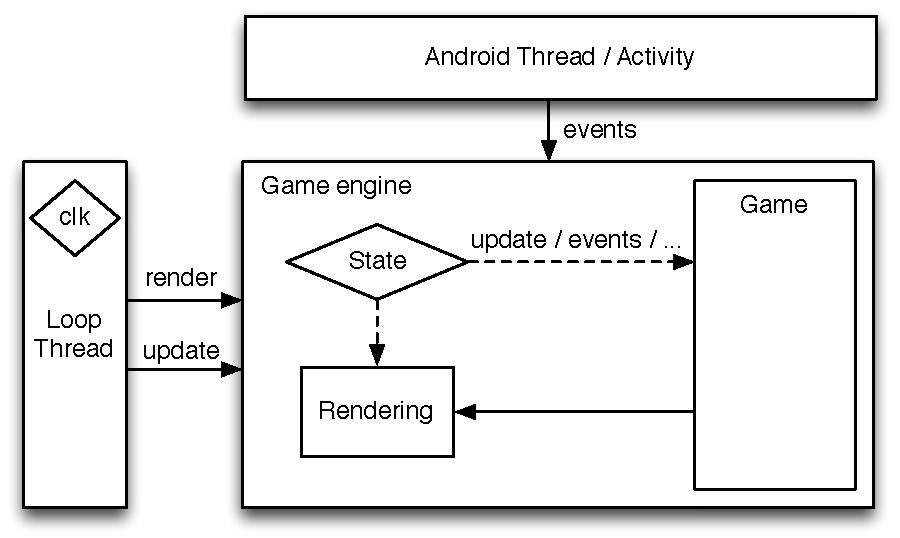
\includegraphics[scale=0.65]{images/architecture-1}
\end{frame}

\begin{frame}{Architecture - 2}
\centering
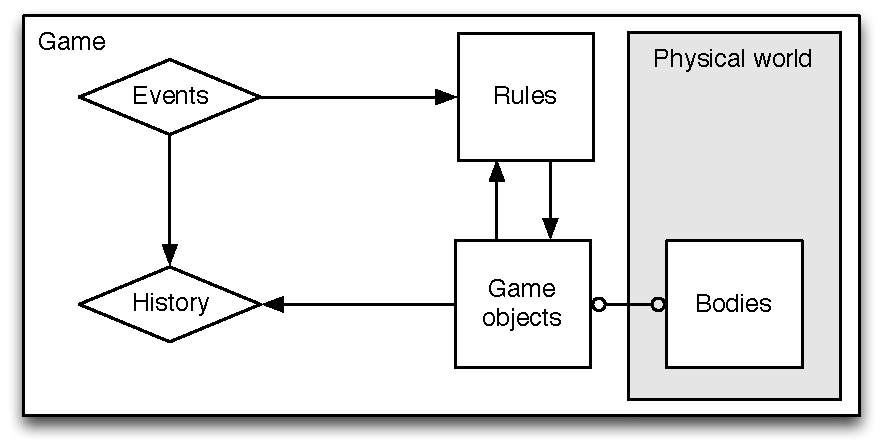
\includegraphics[scale=0.65]{images/architecture-2}
\end{frame}

\begin{frame}[fragile]{Statements and expressions - 1}
\begin{lstlisting}
circle("x") := circle("x") + 1
Assign(circle.x, Add(circle.x, IntegerLiteral(1)))
\end{lstlisting}
\begin{itemize}
\item Permit to modify the rules, the reason about them
\item Use of AST: convenient to manipulate
\item Runtime typechecker and interpreter
\end{itemize}
\end{frame}

\begin{frame}[fragile]{Statements and expressions - 2}
\begin{lstlisting}
circle("x") := circle("x") + 1
\end{lstlisting}
\vspace*{5mm}
\begin{center}
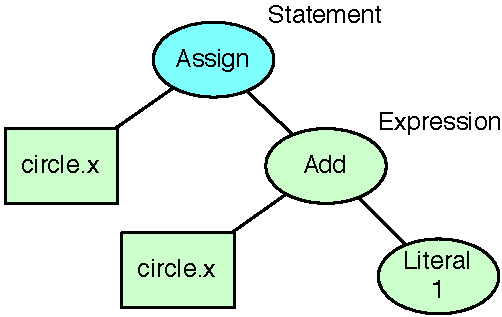
\includegraphics[scale=0.8]{images/AST_example}
\end{center}
\end{frame}


\begin{frame}{Type system}
\begin{itemize}
\item 
\end{itemize}
\end{frame}



\begin{frame}[fragile]{Rules}
\begin{lstlisting}
whenever(Collision(ball, brick)) { Seq(
  brick("visible") := false, 
  score("value") += 1
)}
\end{lstlisting}
\end{frame}

\begin{frame}[fragile]{Categories}
\begin{lstlisting}
val bricks = new Category("Bricks")
rectangle("b1", x = 1, y = 0).withCategory(bricks)
rectangle("b2", x = 3, y = 0).withCategory(bricks)

val rule = foreach(bricks) { brick =>
  whenever(Collision(ball, brick)) { Seq(
    brick("visible") := false,
    score("value") += 1
  )}
}
\end{lstlisting}
\end{frame}


\end{document}